

There are many context where were spatial relationships can be presumed but are not easily established. One
of such fields is in determining a production function in a given state. Traditionally for this problems economic
theory uses a Cobb-Douglas production function \cite{cobb1928theory}. This function model the productivity of a
given economy as a function of labor $(L)$ and capital $(K)$ this can be model is written in the following:

$$
	Y = A K^\alpha L^\beta
$$

Where:
\begin{itemize}
	\item $Y$ is the total output (real GDP) produced.
	\item $A$ is total factor productivity (TFP), capturing the efficiency with which inputs are used.
	\item $K$ is the quantity of physical capital used in production.
	\item $L$ is the quantity of labor employed.
	\item $\alpha$ is the output elasticity of capital, representing the percentage change in output
	      resulting from a 1\% change in capital, holding labor constant.
	\item $\beta$ is the output elasticity of labor, representing the percentage change in output
	      resulting from a 1\% change in labor, holding capital constant.
\end{itemize}

In practice $L,K$ and $Y$ are known and $\alpha$ and $\beta$ are unknown. $\alpha$ and $\beta$ are elasticity factors that ranges
from $0$ and $1$, empirical data shows that healthy economies hover on a labor factor of $0.6$ \cite{douglas1976cobb}.
In the context of local government, these unknown parameters are of interest as they highlight areas where local government
could invest to increase productivity. However as this models are representations of more complex models, it is
reasonable to asume there are some unseen components in our models. An example of this could be the pretense of
informal economies \cite{williams1994spatial}, this referring to transactions that could be reflected in the productivity but can not
be reasonably measured through the official means and this could introduce uncertainty into our model.

Following Econometric theory one could turn Cobb-Douglas equation into a stochastic model \cite{zellner1966specification}.
This can be done in the following format:
\[
	\begin{split}
		Y         & = A K^\alpha L^\beta                                                             \\
		\log{(Y)} & = \log{(A K^\alpha L^\beta)}                                                     \\
		\log(Y)   & = \log(A) + \alpha \log(K) + \beta \log(L) +\epsilon ; \epsilon \sim N(0,\sigma)
	\end{split}
\]



\subsection{Spatial Modeling}

Turning the Cobb-Douglas into a stochastic model that follows the conventual linear regression gives access
to the ability to introduce space into the model. However it is important to define space in this context \cite{paelinck1979spatial}.
Spatial regression models are relatively simple yet expressive tools. The Spatial Durbin Model (SDM) can be expressed as \cite{anselin1998spatial}:

\begin{equation}
	y = X \beta + \rho W X + \epsilon
\end{equation}

In this formulation, $X \beta$ represents the standard linear component, and $\rho W X$ incorporates spatial influence through a known weight
matrix $W$. However, in real-world applications, $W$ is not truly known and must be inferred or chosen by the researcher. For example,
$W$ can be represented in different forms, such as:

\begin{figure}[H]
	\centering
	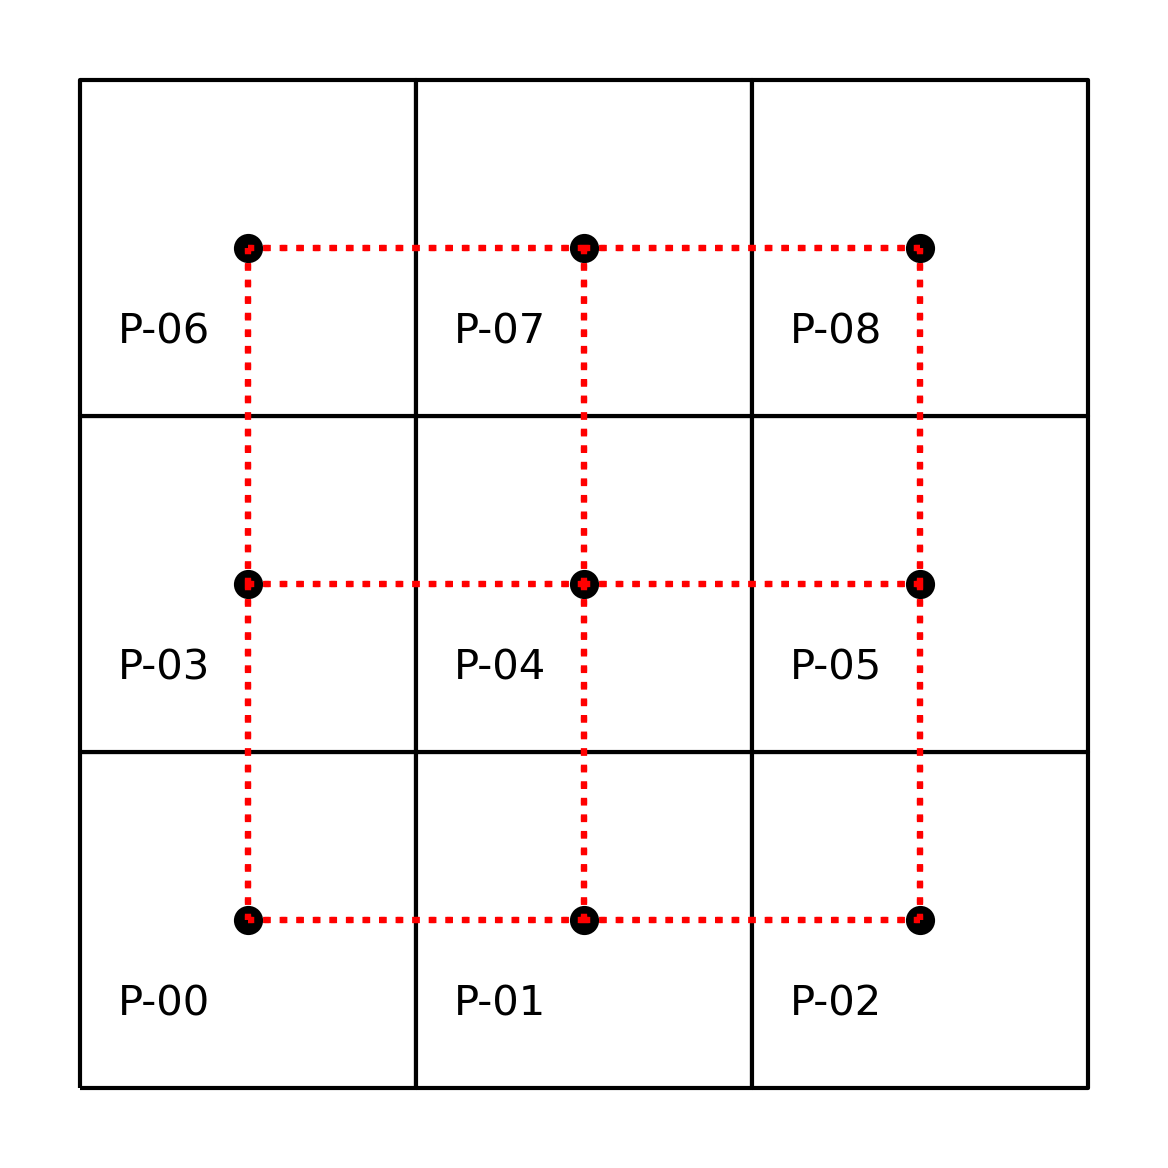
\includegraphics[width=0.4\textwidth]{assets/rook.png}
	\caption{Rook Contiguity Matrix}
\end{figure}

Mathematically, the rook model can be represented as:

\[
	\begin{bmatrix}
		0 & 1 & 0 & 1 & 0 & 0 & 0 & 0 & 0 \\
		1 & 0 & 1 & 0 & 1 & 0 & 0 & 0 & 0 \\
		0 & 1 & 0 & 0 & 0 & 1 & 0 & 0 & 0 \\
		1 & 0 & 0 & 0 & 1 & 0 & 1 & 0 & 0 \\
		0 & 1 & 0 & 1 & 0 & 1 & 0 & 1 & 0 \\
		0 & 0 & 1 & 0 & 1 & 0 & 0 & 0 & 1 \\
		0 & 0 & 0 & 1 & 0 & 0 & 0 & 1 & 0 \\
		0 & 0 & 0 & 0 & 1 & 0 & 1 & 0 & 1 \\
		0 & 0 & 0 & 0 & 0 & 1 & 0 & 1 & 0 \\
	\end{bmatrix}
\]

Another popular variant is the Queen’s contiguity model, which includes all bordering neighbors:

\begin{figure}[H]
	\centering
	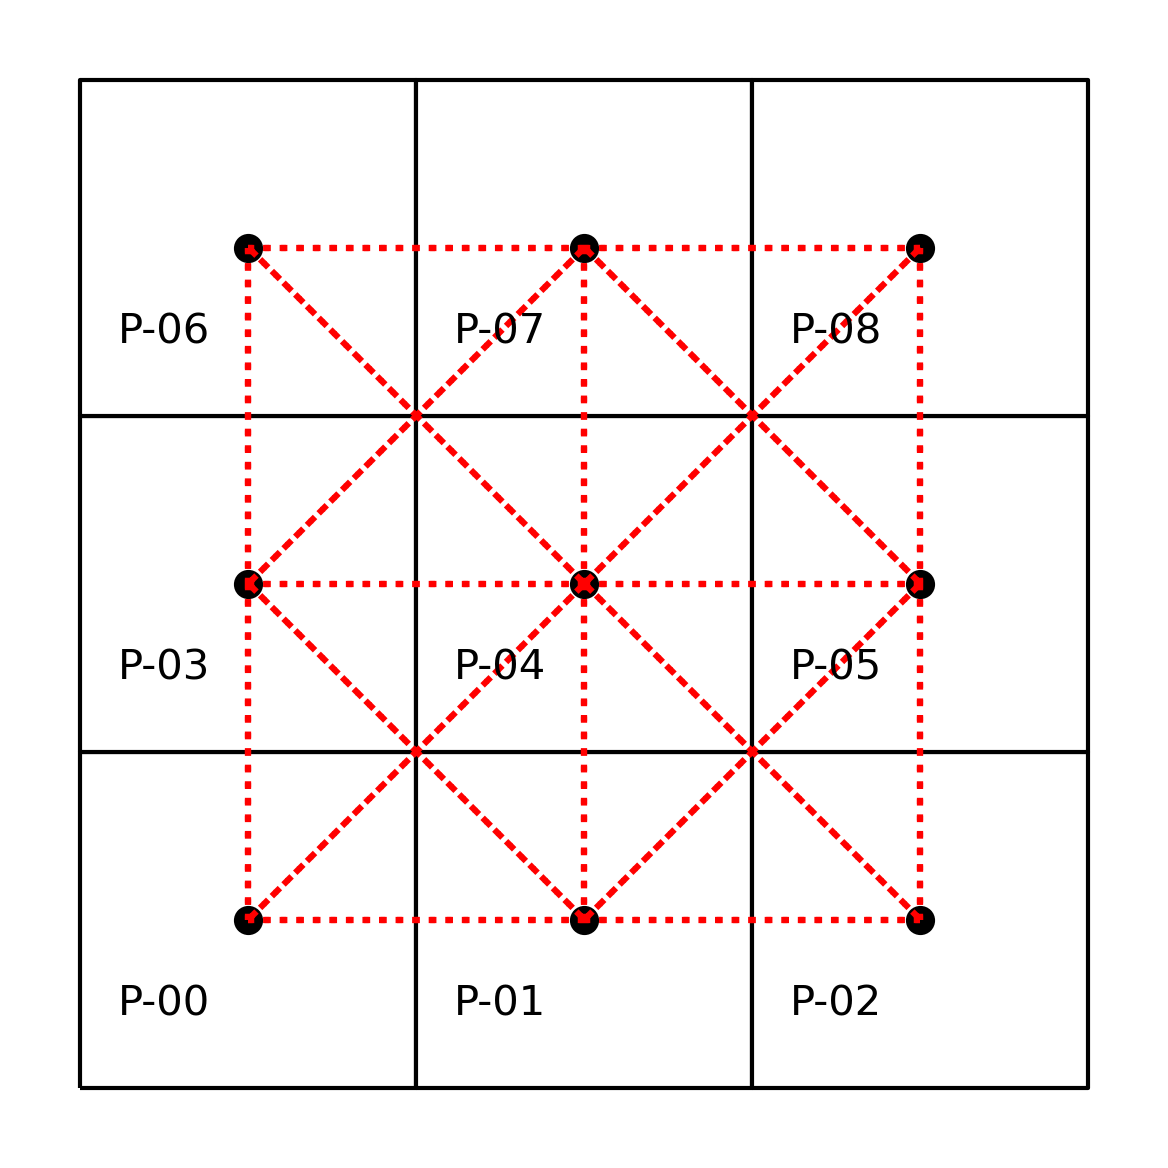
\includegraphics[width=0.4\textwidth]{assets/queens.png}
	\caption{Queen Contiguity Matrix}
\end{figure}

Its corresponding matrix:

\[
	\begin{bmatrix}
		0 & 1 & 0 & 1 & 1 & 0 & 0 & 0 & 0 \\
		1 & 0 & 1 & 1 & 1 & 1 & 0 & 0 & 0 \\
		0 & 1 & 0 & 0 & 1 & 1 & 0 & 0 & 0 \\
		1 & 1 & 0 & 0 & 1 & 0 & 1 & 1 & 0 \\
		1 & 1 & 1 & 1 & 0 & 1 & 1 & 1 & 1 \\
		0 & 1 & 1 & 0 & 1 & 0 & 0 & 1 & 1 \\
		0 & 0 & 0 & 1 & 1 & 0 & 0 & 1 & 0 \\
		0 & 0 & 0 & 1 & 1 & 1 & 1 & 0 & 1 \\
		0 & 0 & 0 & 0 & 1 & 1 & 0 & 1 & 0 \\
	\end{bmatrix}
\]

Another approach is the k-nearest neighbors (KNN) model, where influence decreases with distance \cite{chen2012four}:

\begin{figure}[H]
	\centering
	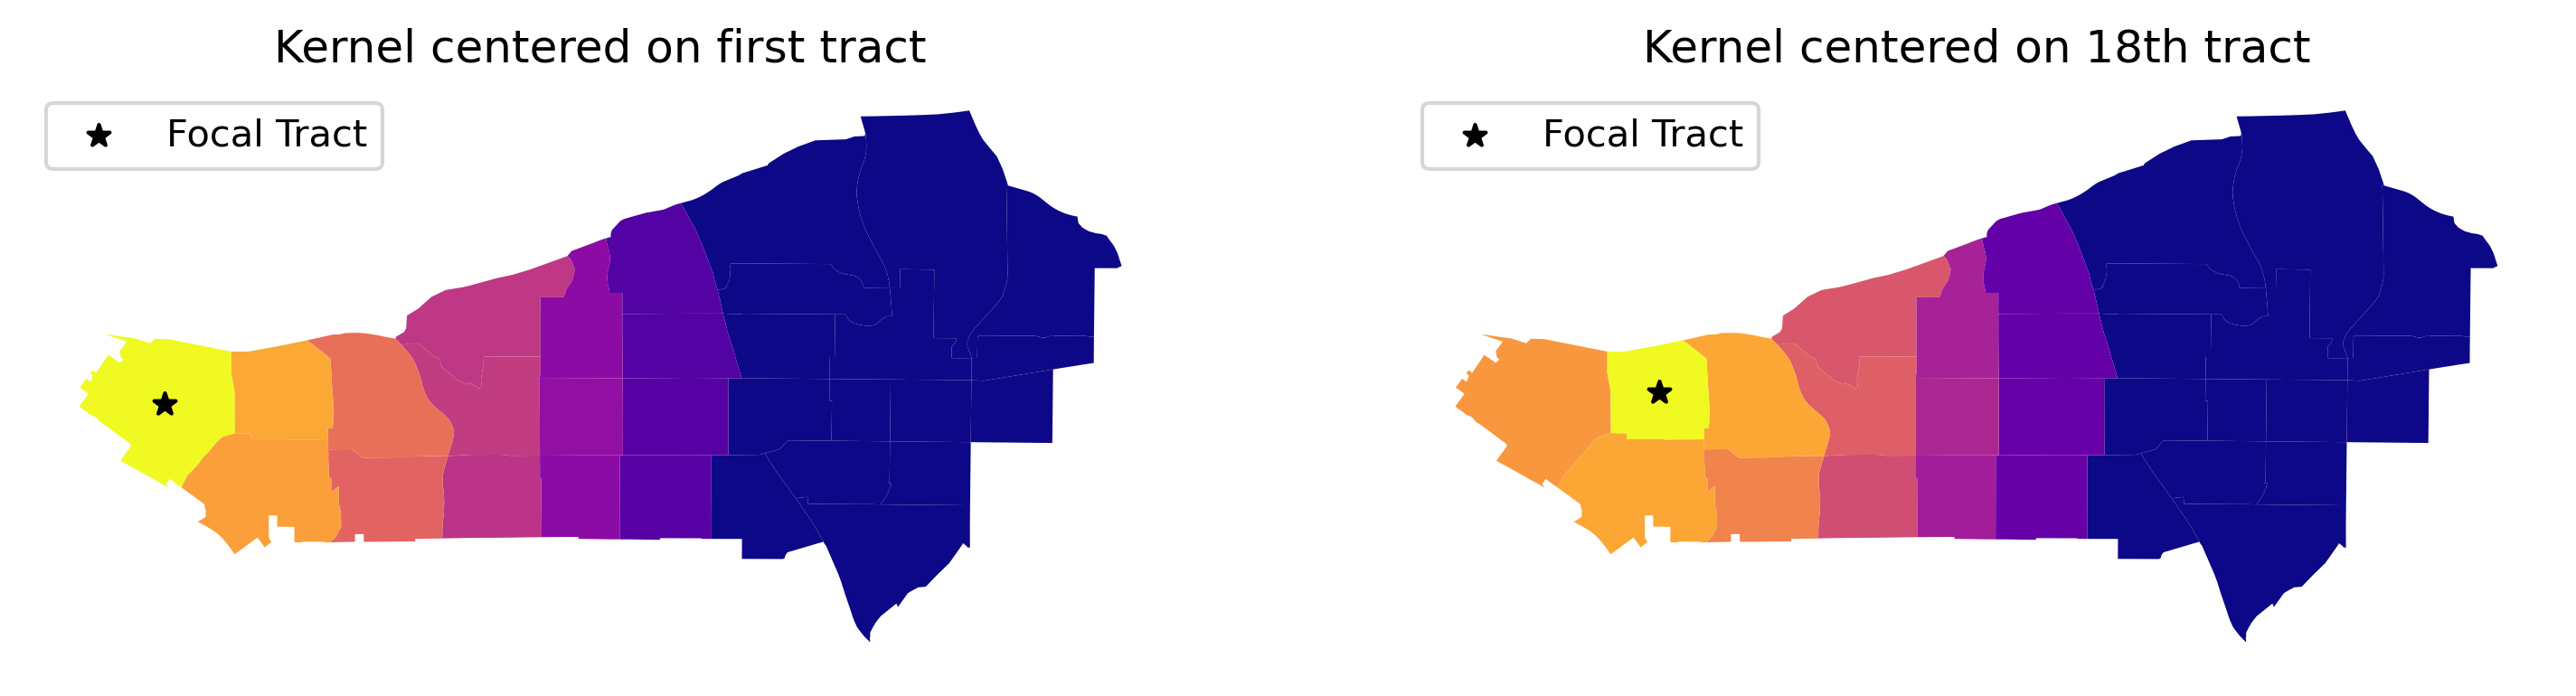
\includegraphics[width=0.64\textwidth]{assets/kmodel.png}
	\caption{K-Nearest Neighbors (KNN) Model}
\end{figure}

Clearly, there are numerous ways to define the $W$ matrix, and no universally accepted method exists for choosing the most
appropriate one. In practice, $W$ is unknown and selecting it remains a major modeling challenge.

\subsection{spatial Cobb-Douglas}

To introduce space into the Cobb-Douglas we tu turn the model into panel. This is can be done building
from what Wang and Henderson showed \cite{wang2022estimation}:
\begin{equation}
	y_{it} = \mu_i + \gamma_t + \alpha k_{it} + \beta l_{it} + \epsilon_{it}
\end{equation}

Where:
\begin{enumerate}[(a)]
	\item $\log(A)_{it} \equiv \mu_i + \gamma_t + \epsilon_{it}$
	\item $\log(L)_{it} \equiv l_{it}$
	\item $\log(K)_{it} \equiv k_{it}$
\end{enumerate}

Contextualizing the panel form of the Cobb-Douglas tell us that you can deconstruct
a given economy into smaller sub economies that share the same elasticities for their labor
and capital but differ in their quantities of capital and labor. Using the notation form the
previos section we can add the spatial component to the Cobb-Douglas function and returning as the orinal function is as follows:
\[
	\begin{split}
		y_{it}       & = \mu_i + \gamma_t + \alpha k_{it} + \beta l_{it} + \rho \sum_{j=1}^N w_{ij} y_{jt} + \epsilon_{it} \\
		\log(Y_{it}) & = \log(A_{it}) + \alpha \log(K_{it}) + \beta \log(L_{it}) + \rho \sum_{j=1}^N w_{ij} \log(Y_{jt})   \\
		Y_{it}       & = A_{it} K^\alpha_{it} L^\beta_{it} \exp \left\{ \rho \sum_{j=1}^N w_{ij} \log(Y_{jt}) \right\}     \\
		Y_{it}       & = A_{it} K^\alpha_{it} L^\beta_{it} e^{\rho \sum_{j=1}^N w_{ij} \log(Y_{jt})}
	\end{split}
\]

\begin{equation}
	Y_{it} = A_{it} K^\alpha_{it} L^\beta_{it} \prod_{j=1}^N Y_{it}^{\rho w_{ij}}
\end{equation}

Introducing space in this way it tell how this smaller economies are affected by the
overall output of neighbors with a given relationship $W$. However as explain previously
there is no universally accepted relationship $W$ and it is possible that depending the
economy looked at this $W$ might be completely different and more complex that would be virtually
imposible to pick an appropriate $W$ for the model. This leads to misspecification \cite{florax2003misspecification}
